\documentclass[t, 				             
			   final, 				         
			   xcolor={usenames,dvipsnames}, 
			   table]{beamer}

% pacotes utilizados.
\usepackage{amsmath}
\usepackage[brazil]{babel}
\usepackage[utf8]{inputenc}
\usepackage{booktabs}
\usepackage[alf]{abntex2cite}
\usepackage{caption}


\usepackage{todo}

% configuração do tema
\usetheme[pageofpages=de,
          bullet=square,			
          titleline=true,				
          alternativetitlepage=true,			
          titlepagelogo=imagens/logo-unicamp,	
          watermarkheight=70px,		
          watermarkheightmult=4	
          ]{Torino}

\setbeamertemplate{sections/subsections in toc}[square]
\setbeamertemplate{bibliography item}[default]

\usecolortheme{freewilly}

\logo{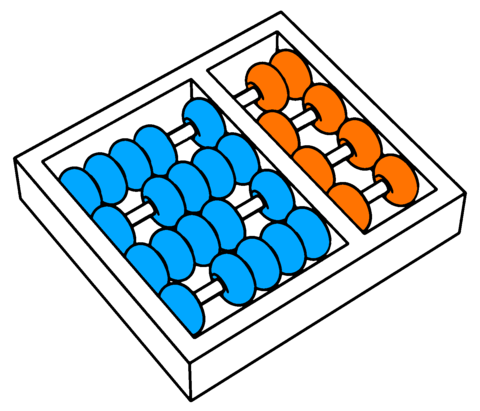
\includegraphics[height=0.110\paperheight]{imagens/logo-ic}}

\begin{document}
    \author{Luiz Alberto Ferreira Gomes}
\title{Manutenibilidade em Linhas de Produtos de Software}
\subtitle{Projeto de Interface de Usuário  }
\institute{Instituto de Computação}
\date{\today}

    \begin{frame}[plain]
  \titlepage
\end{frame}
    \AtBeginSection[]
{
  \begin{frame}{Agenda}
    \tableofcontents[currentsection]
  \end{frame}
}
  
    \section{Primeira Onda}

\begin{frame}[t, fragile]{Primeira Onda}
    \begin{itemize}
    	\item Considerada uma ciência \alert{cognitiva} e relacionada à \alert{fatores humanos}
    	\item Era orientada a modelos e colocava o ser \alert{humano como objeto de estudo}    	
    	\item Por meio de rígidos \alert{guidelines}, métodos formais e testes sistemáticos baseados em métricas
    \end{itemize}  
    \begin{flushright}
		    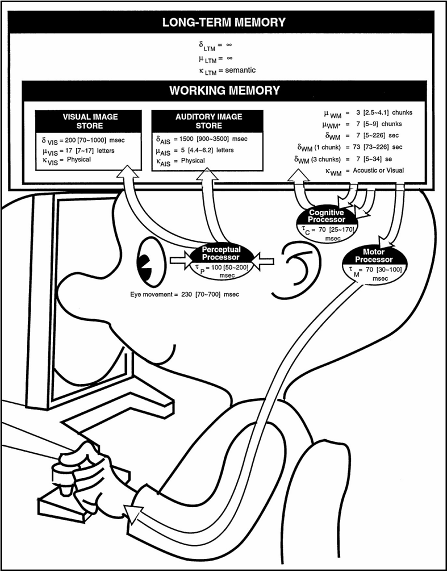
\includegraphics[width=0.25\textwidth]{imagens/primeira-onda}
    \end{flushright} 

\end{frame}
    \section{Segunda Onda}

\begin{frame}[t, fragile]{Segunda Onda}
    \begin{itemize}
    	\item Mudança de "fatores humanos" para "\alert{atores humanos}"
    	\item Foco em \alert{grupos} trabalhando em uma coleção de aplicações.
    	\item Abordagens \alert{qualitativas} e não mais quantitativas, prototipação e design contextual.
    	\item O conceito \alert{contexto}
    	entrou em foco na análise e na interação homem-computador.    
%%    	\item A tecnologia espalho-se do local de trabalho para residências, o dia-a-dia e a cultura.
%    	\item Natureza holística da pessoa em um dado ambiente
    \end{itemize}   
    \begin{flushright}
    	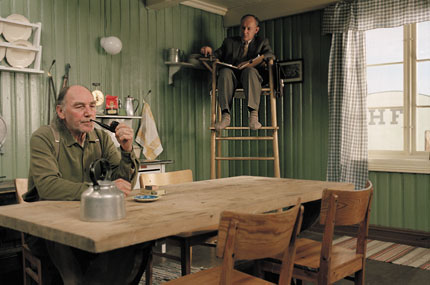
\includegraphics[width=0.45\textwidth]{imagens/segunda-onda}
    \end{flushright}
\end{frame}
	\section{Terceira Onda}

\begin{frame}[t, fragile]{Terceira Onda}
    \begin{itemize}
    	\item Foco em aspectos culturais e estéticos
    	\item Expansão do cognitivo ao \alert{emocional}
    	\item Fatores pragmáticos \alert{sociais} da experiência 
    	\item Tecnologias \alert{ubíquas}, móveis e pequenas.
		\item A tecnologia espalho-se do local de \alert{trabalho} para \alert{residências}, o dia-a-dia e a cultura.
    \end{itemize}   
     \begin{flushright}
     	
\includegraphics[width=0.20\textwidth]{imagens/terceira-onda}
     \end{flushright}
\end{frame}
	\section{Produto Exemplo}
\begin{frame}[allowframebreaks, t, fragile]{Produto: Sistema de Gestão de Manutenção}
	\begin{columns}
	  	\begin{column}{0.45\textwidth}
	  		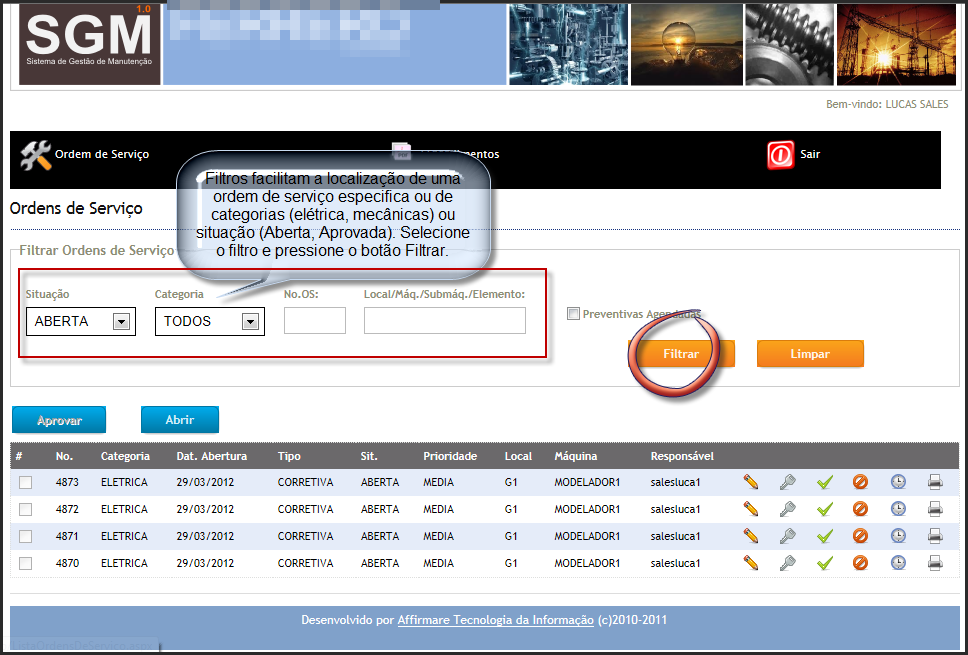
\includegraphics[width=1\textwidth]{imagens/sgm-01}
	  	\end{column}
	  	\begin{column}{0.45\textwidth}
	  		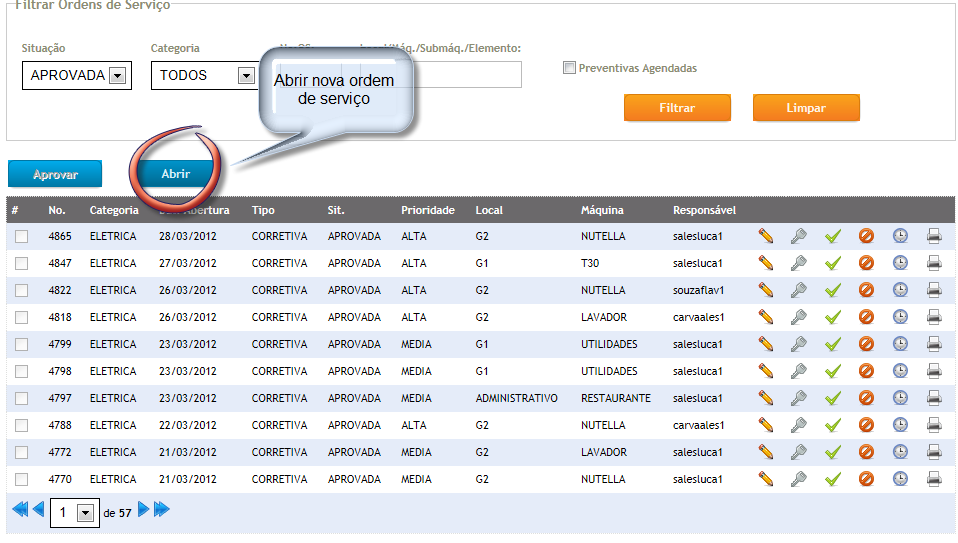
\includegraphics[width=1\textwidth]{imagens/sgm-02}
	  	\end{column}
	\end{columns}

	\begin{itemize}
		\item Sistema para gestão da manutenção dos equipamentos e máquinas de uma fábrica
		\item Entrou em operação em 2010 e foi aposentado no final de 2015.
	\end{itemize}

	\framebreak
	
%	\begin{columns}
%		\begin{column}{0.45\textwidth}
%			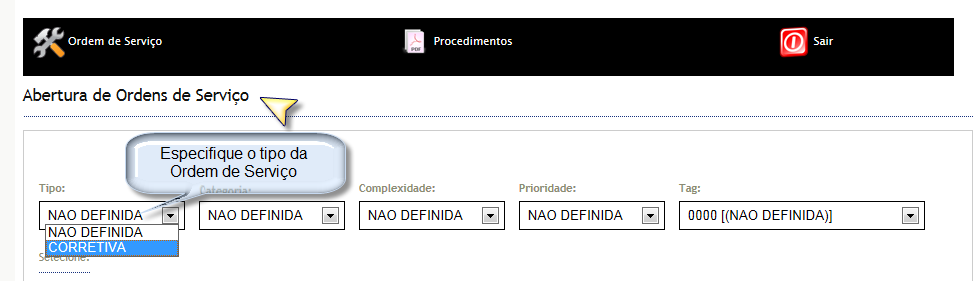
\includegraphics[width=1\textwidth]{imagens/sgm-03}
%		\end{column}
%		\begin{column}{0.45\textwidth}
%			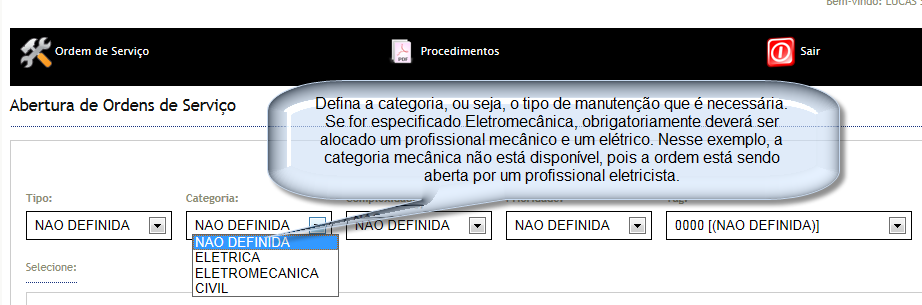
\includegraphics[width=1\textwidth]{imagens/sgm-04}
%		\end{column}
%	\end{columns}
	

		
%	\framebreak
	
	\begin{columns}
		\begin{column}{0.45\textwidth}
			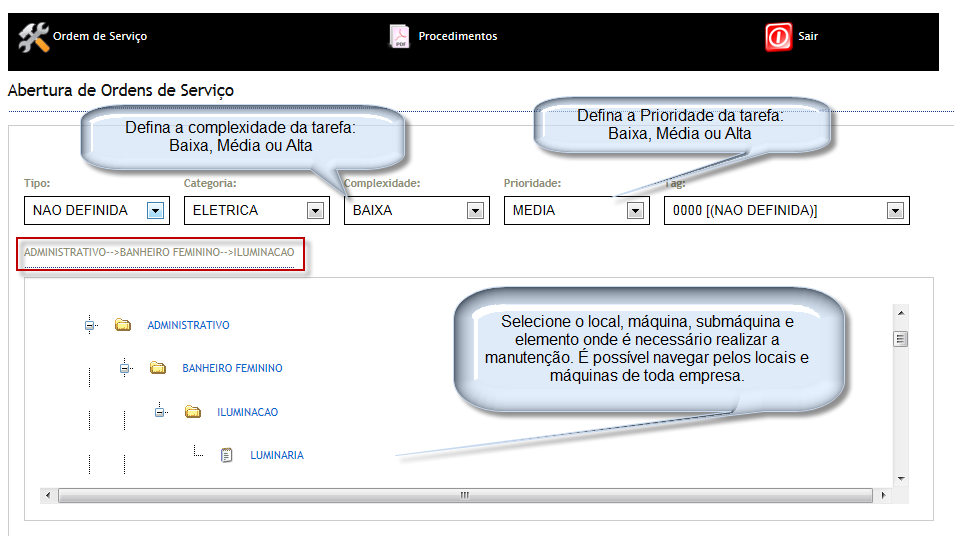
\includegraphics[width=1\textwidth]{imagens/sgm-05}
		\end{column}
		\begin{column}{0.45\textwidth}
			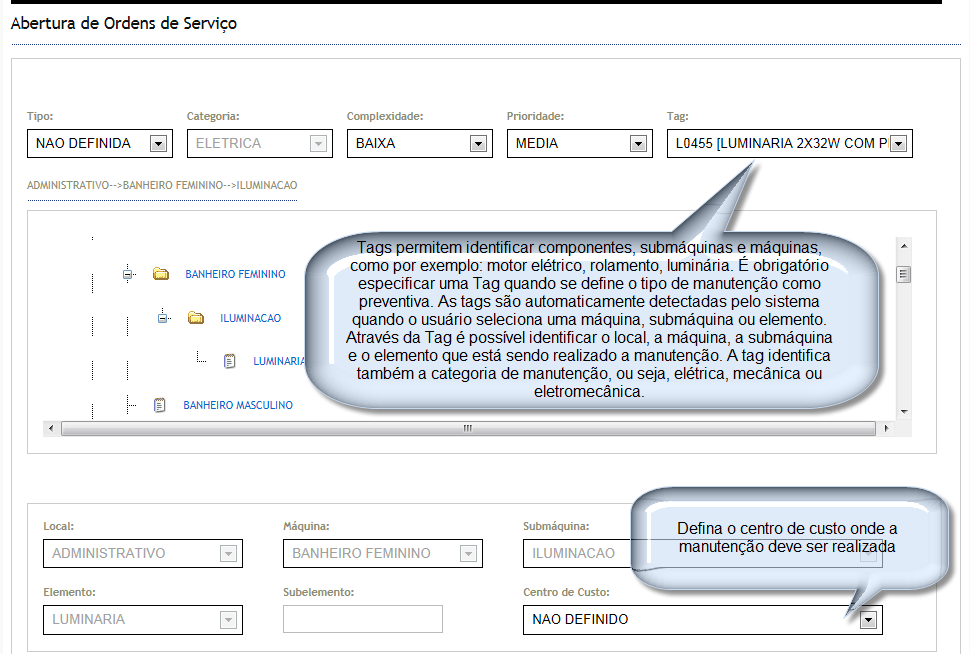
\includegraphics[width=1\textwidth]{imagens/sgm-06}
		\end{column}
	\end{columns}
	
	\begin{itemize}
		\item \textbf{Problemas com a primeira onda}:
		\begin{itemize}
			\item Não apresenta um \alert{guia consistente} de elementos da interface 
			\item Usabilidade \alert{pobre} (por exemplo: feedbacks não são claros dificultando o aprendizado)
		\end{itemize}
	\end{itemize}
		
	\framebreak
		
		\begin{columns}
			\begin{column}{0.45\textwidth}
				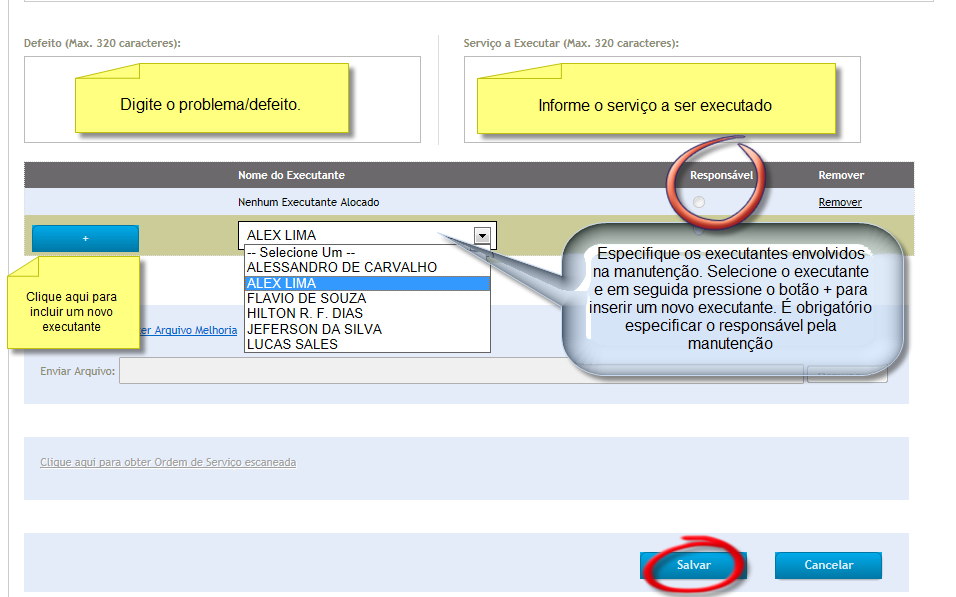
\includegraphics[width=1\textwidth]{imagens/sgm-07}
			\end{column}
			\begin{column}{0.45\textwidth}
				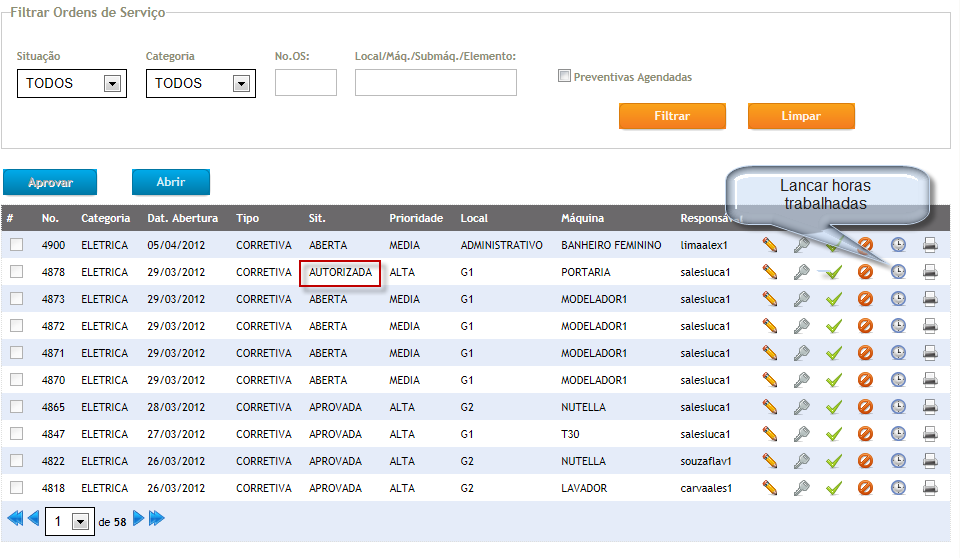
\includegraphics[width=1\textwidth]{imagens/sgm-08}
			\end{column}
		\end{columns}

	\begin{itemize}
		\item \textbf{Problemas com a segunda onda}:
		\begin{itemize}
			\item \alert{Contextos diferentes} NÃO \underline{foram levados em consideração}: a manutenção pode ocorrer no escritório e na linha de produção; pode ser elétrica ou mecânica etc. 
		\end{itemize}
	\end{itemize}
		
	\framebreak
	
	\begin{columns}
		\begin{column}{0.45\textwidth}
			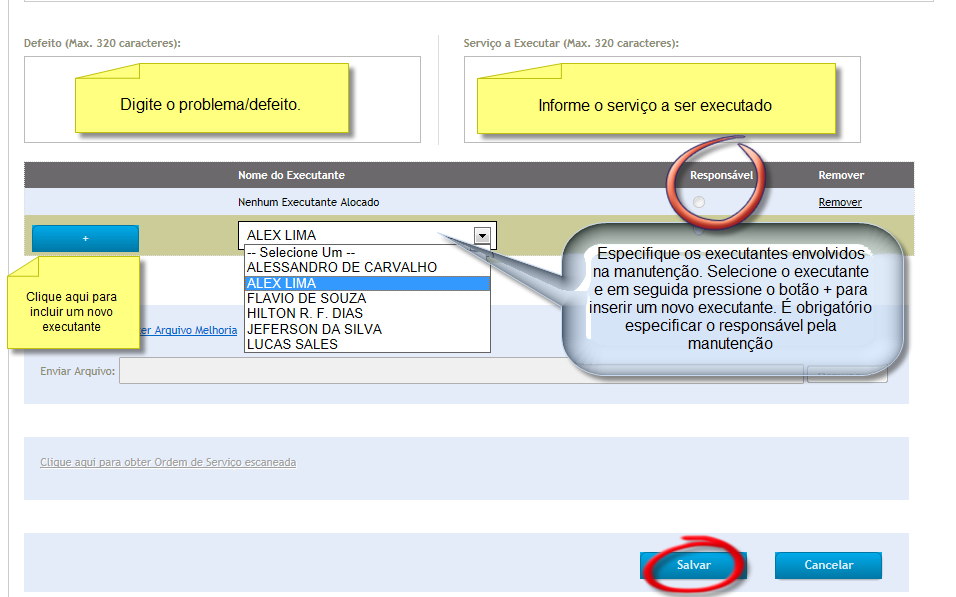
\includegraphics[width=1\textwidth]{imagens/sgm-07}
		\end{column}
		\begin{column}{0.45\textwidth}
			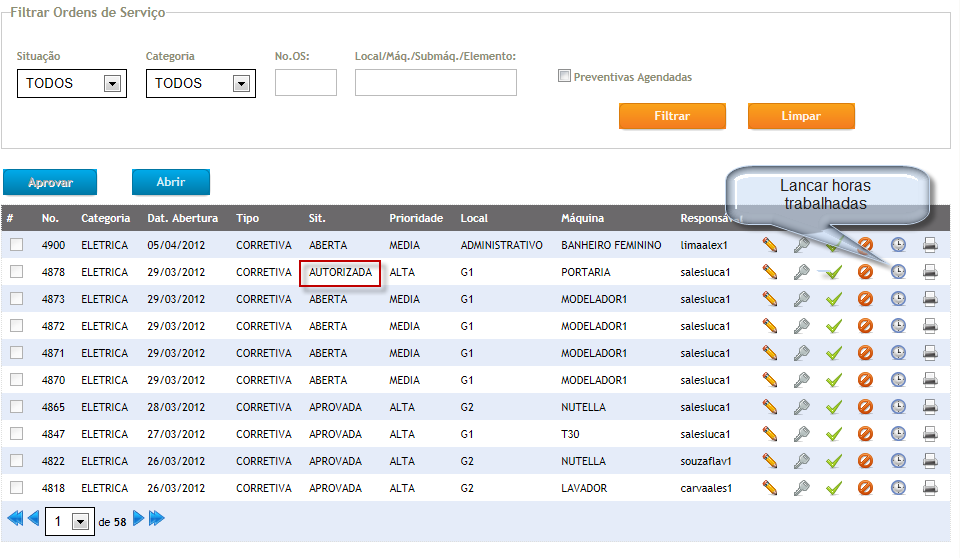
\includegraphics[width=1\textwidth]{imagens/sgm-08}
		\end{column}
	\end{columns}
	
	\begin{itemize}
		\item \textbf{Problemas com a terceira onda}:
		\begin{itemize}
			\item Não há uma \alert{interface móvel} para facilitar o acesso ao sistema.
			\item A \alert{estética} \underline{deixa muito a desejar}.
			\item Não existe metáforas que promovam uma \alert{ligação psicológica} com os usuários.
			 
		\end{itemize}
	\end{itemize}

	
\end{frame}
%    \section{Produto Exemplo}
\begin{frame}[allowframebreaks, t, fragile]{Produto: Sistema de Gestão de Manutenção}
	\begin{columns}
	  	\begin{column}{0.45\textwidth}
	  		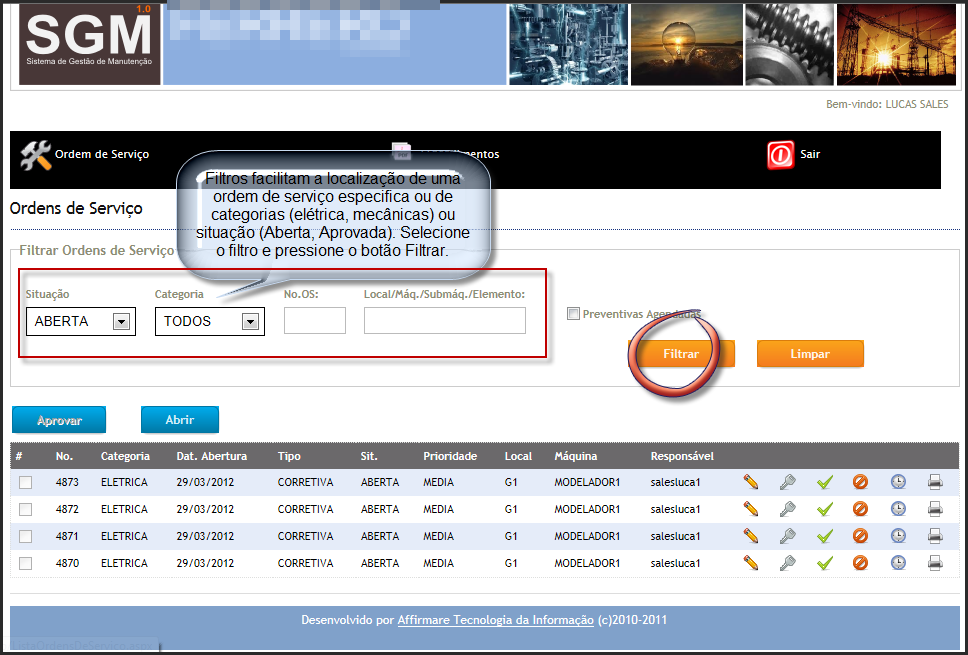
\includegraphics[width=1\textwidth]{imagens/sgm-01}
	  	\end{column}
	  	\begin{column}{0.45\textwidth}
	  		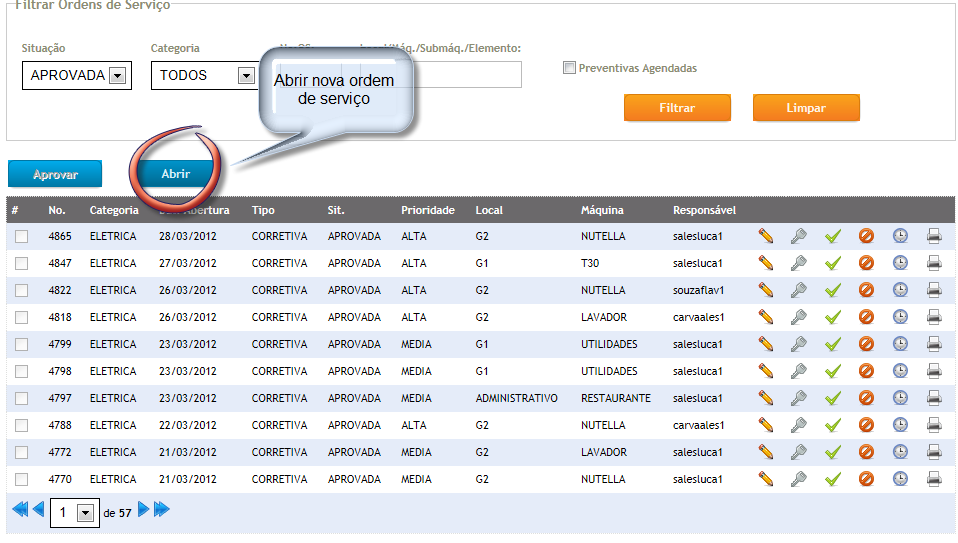
\includegraphics[width=1\textwidth]{imagens/sgm-02}
	  	\end{column}
	\end{columns}



	\framebreak
	
	\begin{columns}
		\begin{column}{0.45\textwidth}
			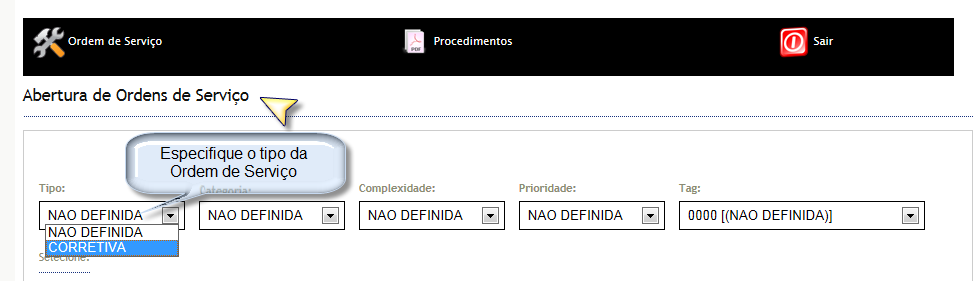
\includegraphics[width=1\textwidth]{imagens/sgm-03}
		\end{column}
		\begin{column}{0.45\textwidth}
			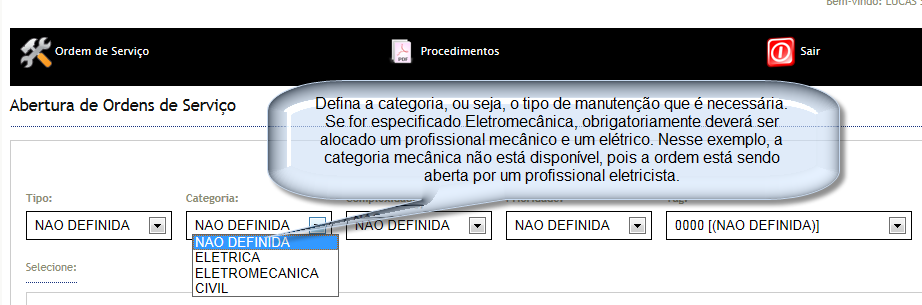
\includegraphics[width=1\textwidth]{imagens/sgm-04}
		\end{column}
	\end{columns}
	
	\framebreak
	
	\begin{columns}
		\begin{column}{0.45\textwidth}
			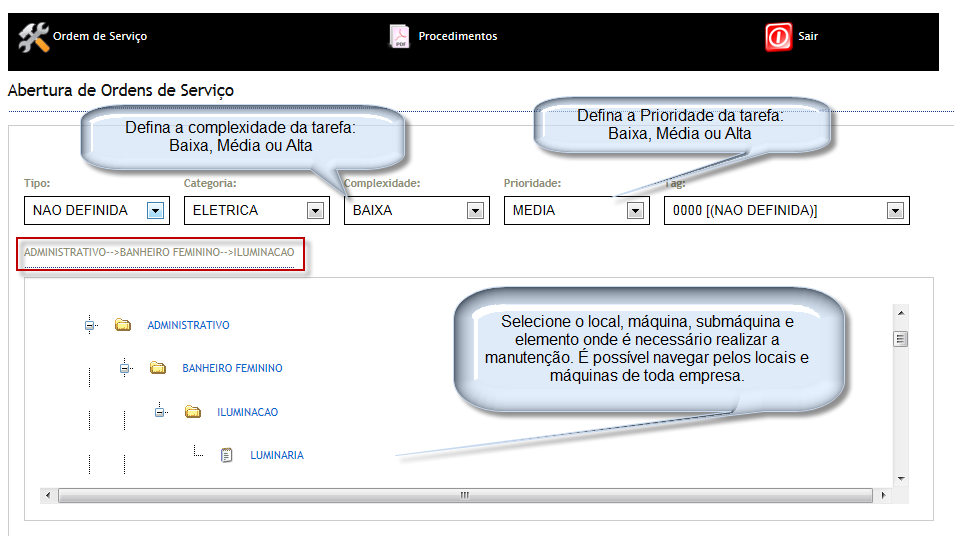
\includegraphics[width=1\textwidth]{imagens/sgm-05}
		\end{column}
		\begin{column}{0.45\textwidth}
			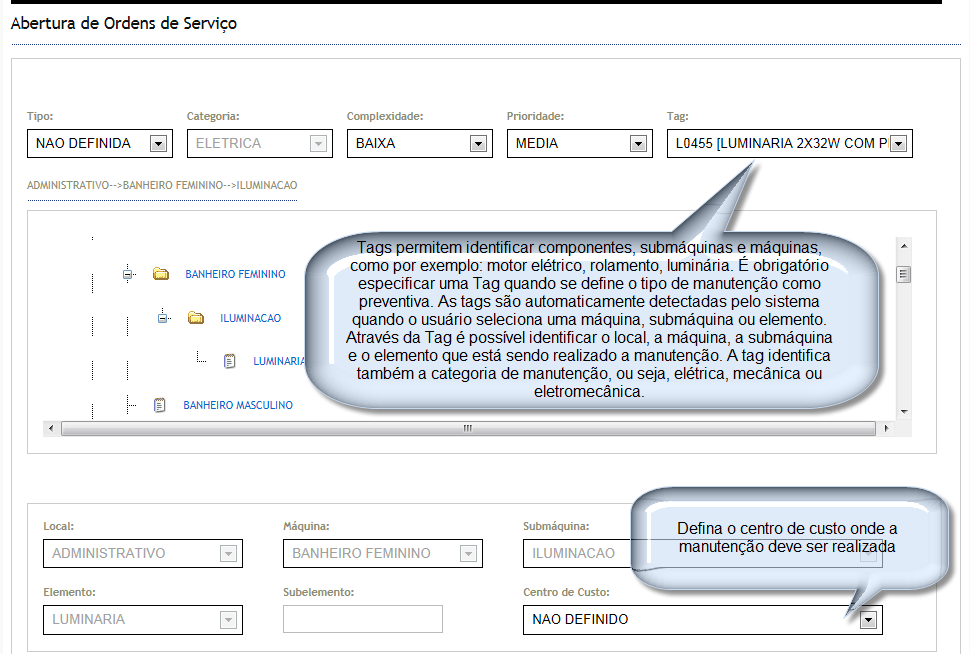
\includegraphics[width=1\textwidth]{imagens/sgm-06}
		\end{column}
	\end{columns}
	
	\framebreak
		
		\begin{columns}
			\begin{column}{0.45\textwidth}
				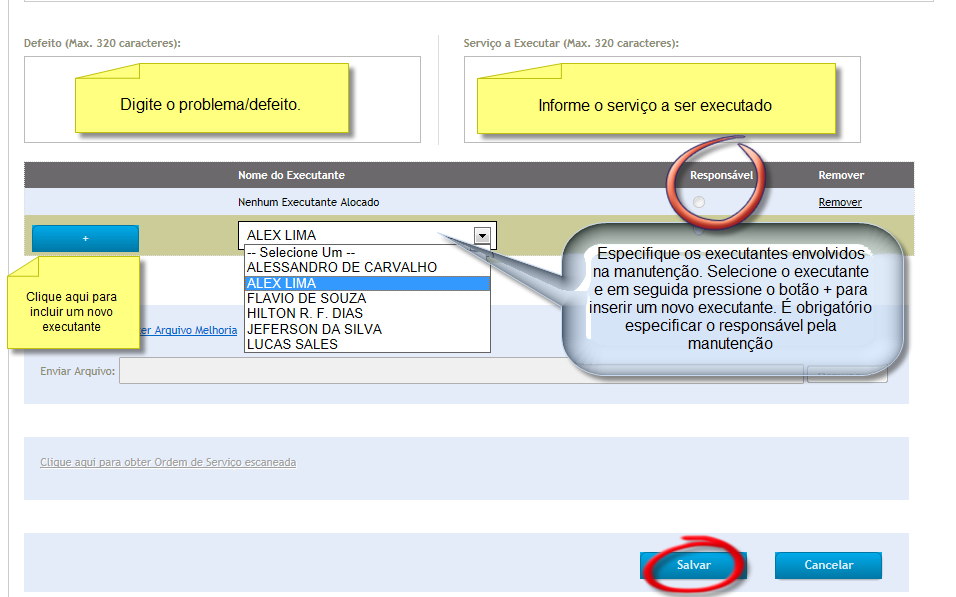
\includegraphics[width=1\textwidth]{imagens/sgm-07}
			\end{column}
			\begin{column}{0.45\textwidth}
				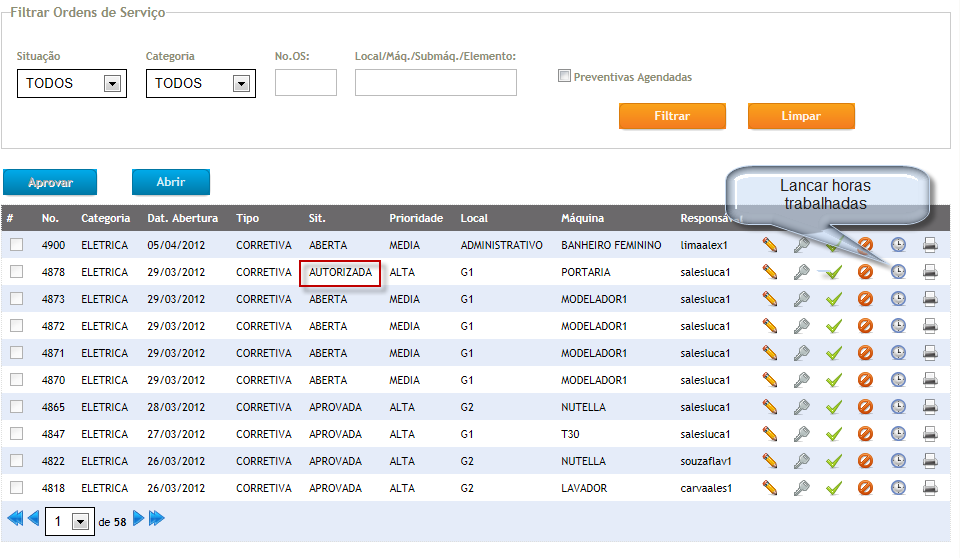
\includegraphics[width=1\textwidth]{imagens/sgm-08}
			\end{column}
		\end{columns}

	\framebreak
	
	\begin{columns}
		\begin{column}{0.45\textwidth}
			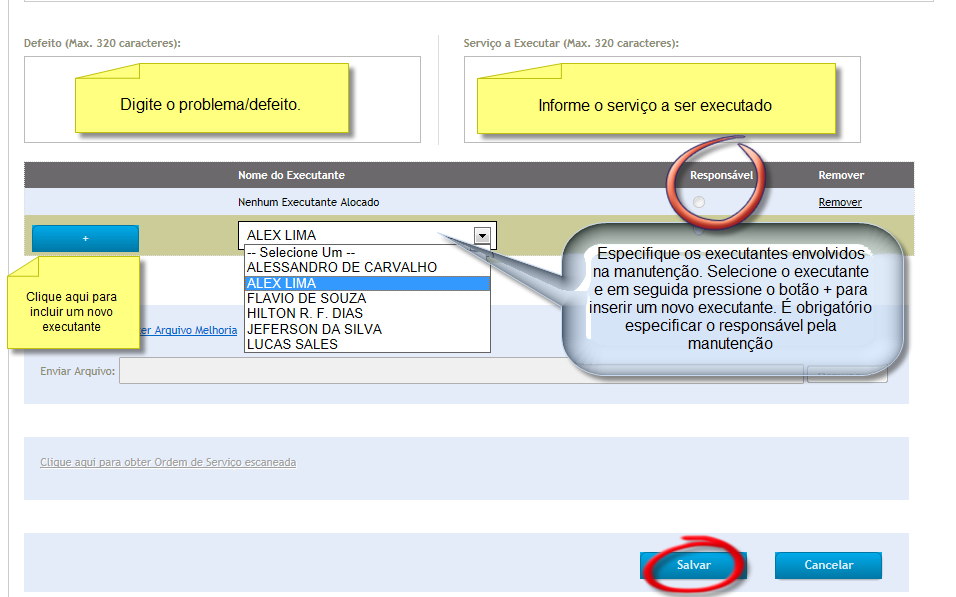
\includegraphics[width=1\textwidth]{imagens/sgm-07}
		\end{column}
		\begin{column}{0.45\textwidth}
			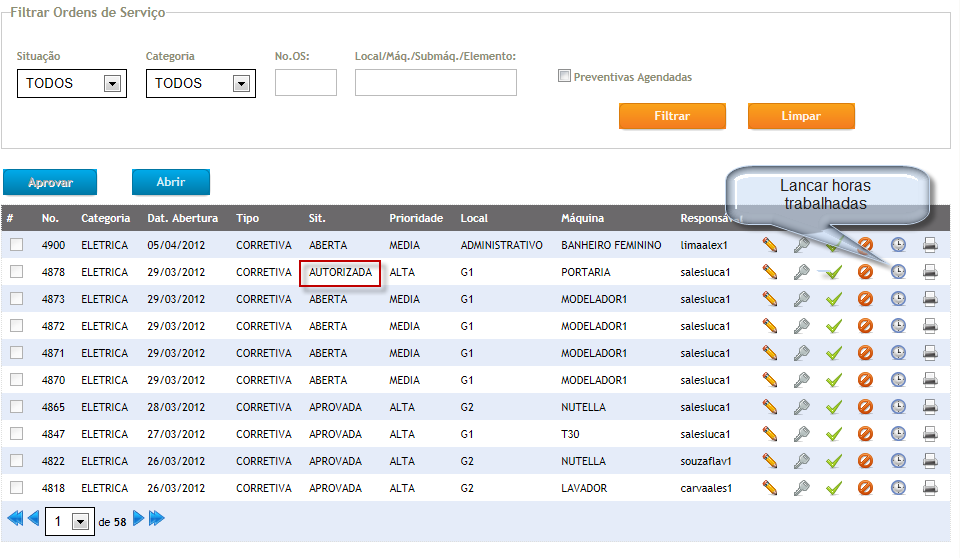
\includegraphics[width=1\textwidth]{imagens/sgm-08}
		\end{column}
	\end{columns}
	
\end{frame}
    \nocite{Bodker:2006}
\nocite{Bodker:2015}

    \section{Bibliografia}
\begin{frame}[t, fragile]{Bibliografia}
	\bibliography{Bibliografia}
\end{frame}

\end{document}

